\begin{section}{RM}{Dark Galaxy Candidates at Redshift ~3.5 Detected with MUSE}
  \begin{minipage}[l]{\textwidth}

    {\small Recent theoretical models suggest that the early phase of galaxy
      formation involves an epoch when galaxies are gas-rich but inefficient
      at forming stars: a ``dark galaxy'' phase. We perform an integral field
      survey for dark galaxies fluorescently illuminated by quasars at z>3
      with MUSE, which provides us a nearly uniform sensitvity coverage over a
      large volume in redshift space, compared to previous narrow-band imaging
      surveys. By comparing the rest-frame equivalent width (EW\_0)
      distributions of the Lyalpha sources detected in proximity to the
      quasars and in control samples, we detect a clear correlation between
      the locations of high EW\_0 objects and the quasars, not seen in other
      properties such as Lyalpha luminosities or volume overdensities,
      suggesting the possible fluorescent nature of at least some of these
      objects. Among these, we found 6 dark galaxy candidates with EW\_0 limits
      larger than 240 Angstrom with similar properties to previously detected
      candidates at z~2.4. Our results also provide a lower limit of 60 Myr on
      the quasar lifetime.}
  \end{minipage}

  \vspace{0.5cm}

  \begin{minipage}{\linewidth}
    \begin{center}
      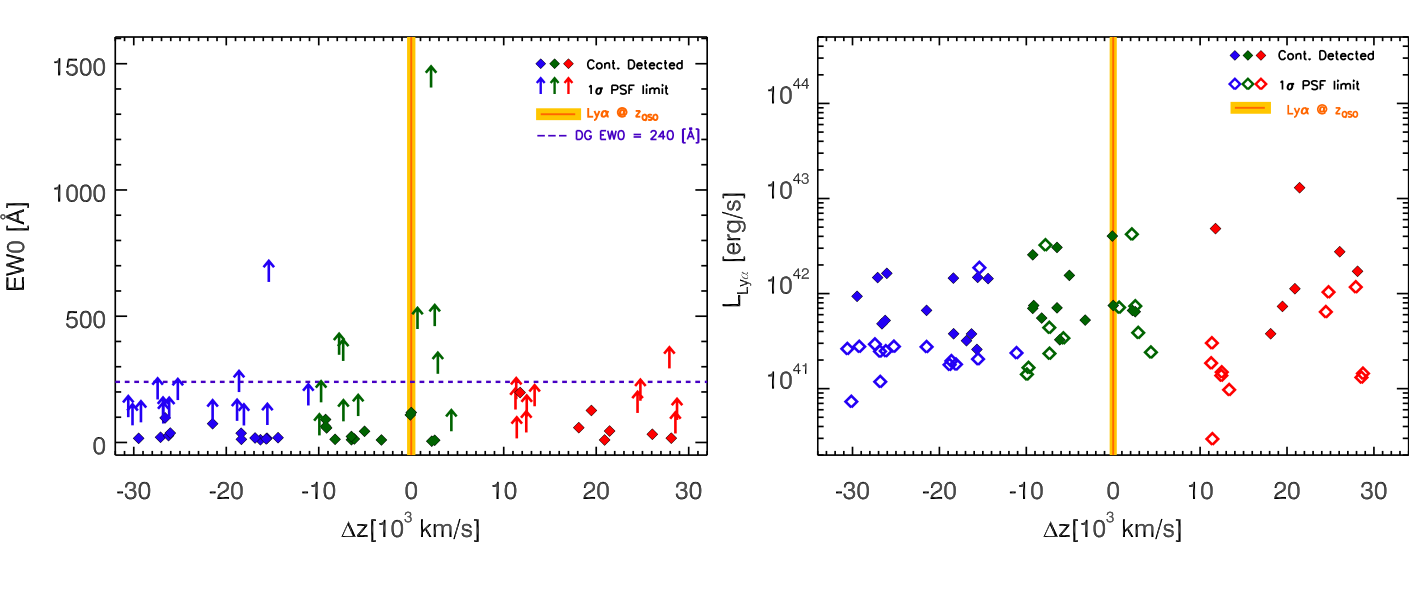
\includegraphics[height=10cm]{RM/EW_LUM_highz.png}
    \end{center}
  \end{minipage}

  \vspace{0.5cm}

  {\footnotesize \textit{[Marino, Raffaella Anna et al. 2017, arXiv:1709.03522]}}
\end{section}